\subsection{A Finite Element Approach to Imaging}

Consequently, our research presents novel FEM and computational methods to model and explore AFM images, specifically in biomolecular samples. The primary work of this research focuses on improving the modelling of previous AFM simulations from a hard sphere model to a model with tip surface interactions. FEM simulations enable us to simulate tip indentation and generate force curves that incorporate more intricate forces and dynamics. We employ several FEM simulations to investigate contact models of indentation and sample compression in AFM imaging. The overall goal was to produce more accurate images and artefacts. 

FEM subdivides the geometry into small, discrete finite elements, producing a surface mesh as shown in Figure \ref{fig: FEM model}. The dynamics are approximated over these finite elements and result in a system of algebraic equations. The system is then modelled using the assembled equations for the finite elements and solutions are approximated via the calculus of variations and minimising an associated error function. Producing AFM images requires the calculation of contours of constant indentation force. Using FEM, the sample surface and probe tip geometry are recreated, and individual indentations across the sample are simulated. This provides 4-dimensional arrays of indenter position and corresponding indentation force. From this, contours of constant force can be used to return the surface contour.


\begin{figure}[H]
    \centering
    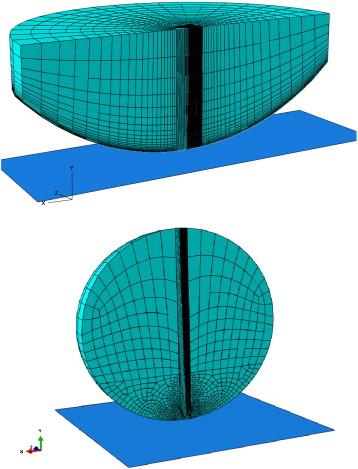
\includegraphics[trim = 0 0 0 130, clip, width=0.38\linewidth]{Figures/FEM mode.jpg}
    \caption{Graphic of FEM mesh for a simulation of sphere indentation by Zheng \textit{et al.}\cite{zheng2012finite}}
    \label{fig: FEM model}
\end{figure}


Our implementation of FEM utilises the commercial engineering software ABAQUS. However, as ABAQUS is an engineering-focused software and simulating biological AFM imaging is a novel application for ABAQUS, initial tests verified its viability. The accuracy of ABAQUS was evaluated through tests that focused on elastic indentation, performed on both elastic half-spaces with varying depths and elastic spheres with varying radii. These tests are outlined in Section \ref{Chapter 2: ABAQUS Applied to Contact Models}. Following these initial simulations, a FEM approach was applied to produce simulations of the AFM raster-scanning dynamic, outlined in Section \ref{Chapter 2: ABAQUS Simulation of AFM Raster Scan}. These simulations were used to analyse the compression of a simple hemisphere and periodic surfaces (Section \ref{Chapter 2: Quantitative Analysis of Surface Compression}). Finally, a FEM approach was applied to simulate the AFM appearance of simple biomolecules, outlined in Section \ref{Chapter 2: ABAQUS Simulation of AFM Biomolecules}. 